\let\negmedspace\undefined
\let\negthickspace\undefined
\documentclass[journal,12pt]{IEEEtran}
\usepackage[a5paper, margin=10mm, onecolumn]{geometry}
\usepackage{tfrupee}

\setlength{\headheight}{1cm}
\setlength{\headsep}{0mm}

\usepackage{gvv-book}
\usepackage{gvv}
\usepackage{cite}
\usepackage{amsmath,amssymb,amsfonts,amsthm}
\usepackage{algorithmic}
\usepackage{graphicx}
\usepackage{textcomp}
\usepackage{xcolor}
\usepackage{txfonts}
\usepackage{listings}
\usepackage{enumitem}
\usepackage{mathtools}
\usepackage{gensymb}
\usepackage{comment}
\usepackage[breaklinks=true]{hyperref}
\usepackage{tkz-euclide}
\usepackage{float}
\def\inputGnumericTable{}
\usepackage[latin1]{inputenc}
\usepackage{color}
\usepackage{array}
\usepackage{longtable}
\usepackage{calc}
\usepackage{multirow}
\usepackage{hhline}
\usepackage{ifthen}
\usepackage{lscape}

\begin{document}

\bibliographystyle{IEEEtran}
\vspace{2cm}

\title{5.5.17}
\author{EE25BTECH11065 - Yoshita J}

{\let\newpage\relax\maketitle}

\renewcommand{\thefigure}{\theenumi}
\renewcommand{\thetable}{\theenumi}
\setlength{\intextsep}{10pt}

\textbf{Question}\\
If 

\[
\vec{A} = 
\myvec{
1 & 1 & 1\\
0 & 1 & 3\\
1 & -2 & 1
},
\]

find \( \vec{A}^{-1} \) using elementary row transformations. Hence, solve the system:
\begin{align*}
x + y + z &= 6\\
y + 3z &= 11\\
x - 2y + z &= 0
\end{align*}

\textbf{Solution:}

\begin{align}
\vec{A} = 
\begin{pmatrix}
1 & 1 & 1\\
0 & 1 & 3\\
1 & -2 & 1
\end{pmatrix}
\end{align}

The augmented matrix is:
\begin{align}
\augvec{3}{3}{
1 & 1 & 1 & 1 & 0 & 0 \\
0 & 1 & 3 & 0 & 1 & 0 \\
1 & -2 & 1 & 0 & 0 & 1
}
\end{align}

Row operations:

\begin{align}
R_3 \to R_3 - R_1 &\Rightarrow 
\augvec{3}{3}{
1 & 1 & 1 & 1 & 0 & 0 \\
0 & 1 & 3 & 0 & 1 & 0 \\
0 & -3 & 0 & -1 & 0 & 1
}
\\
R_3 \to R_3 + 3R_2 &\Rightarrow 
\augvec{3}{3}{
1 & 1 & 1 & 1 & 0 & 0 \\
0 & 1 & 3 & 0 & 1 & 0 \\
0 & 0 & 9 & -1 & 3 & 1
}
\\
R_3 \to \frac{1}{9}R_3 &\Rightarrow 
\augvec{3}{3}{
1 & 1 & 1 & 1 & 0 & 0 \\
0 & 1 & 3 & 0 & 1 & 0 \\
0 & 0 & 1 & -\frac{1}{9} & \frac{1}{3} & \frac{1}{9}
}
\\
R_1 \to R_1 - R_3,\quad R_2 \to R_2 - 3R_3 &\Rightarrow 
\augvec{3}{3}{
1 & 1 & 0 & \frac{10}{9} & -\frac{1}{3} & -\frac{1}{9} \\
0 & 1 & 0 & \frac{1}{3} & 0 & -\frac{1}{3} \\
0 & 0 & 1 & -\frac{1}{9} & \frac{1}{3} & \frac{1}{9}
}
\\
R_1 \to R_1 - R_2 &\Rightarrow 
\augvec{3}{3}{
1 & 0 & 0 & \frac{7}{9} & -\frac{1}{3} & \frac{2}{9} \\
0 & 1 & 0 & \frac{1}{3} & 0 & -\frac{1}{3} \\
0 & 0 & 1 & -\frac{1}{9} & \frac{1}{3} & \frac{1}{9}
}
\end{align}

As the left block becomes identity, the right block is \( \vec{A}^{-1} \):

\begin{align}
\vec{A}^{-1} = 
\myvec{
\frac{7}{9} & -\frac{1}{3} & \frac{2}{9}\\
\frac{1}{3} & 0 & -\frac{1}{3}\\
-\frac{1}{9} & \frac{1}{3} & \frac{1}{9}
}
\end{align}

Now solving: \quad \( \vec{x} = \vec{A}^{-1} \vec{b} \), where
\[
\vec{b} = 
\myvec{
6\\
11\\
0
}
\]

\begin{align}
\vec{x} = 
\myvec{
\frac{7}{9} & -\frac{1}{3} & \frac{2}{9}\\
\frac{1}{3} & 0 & -\frac{1}{3}\\
-\frac{1}{9} & \frac{1}{3} & \frac{1}{9}
}
\myvec{
6\\
11\\
0
}
=
\myvec{
1\\
2\\
3
}
\end{align}

\textbf{Final Answer:}
\begin{align}
\boxed{x = 1,\quad y = 2,\quad z = 3}
\end{align}

\begin{figure}[h!]
\begin{center}
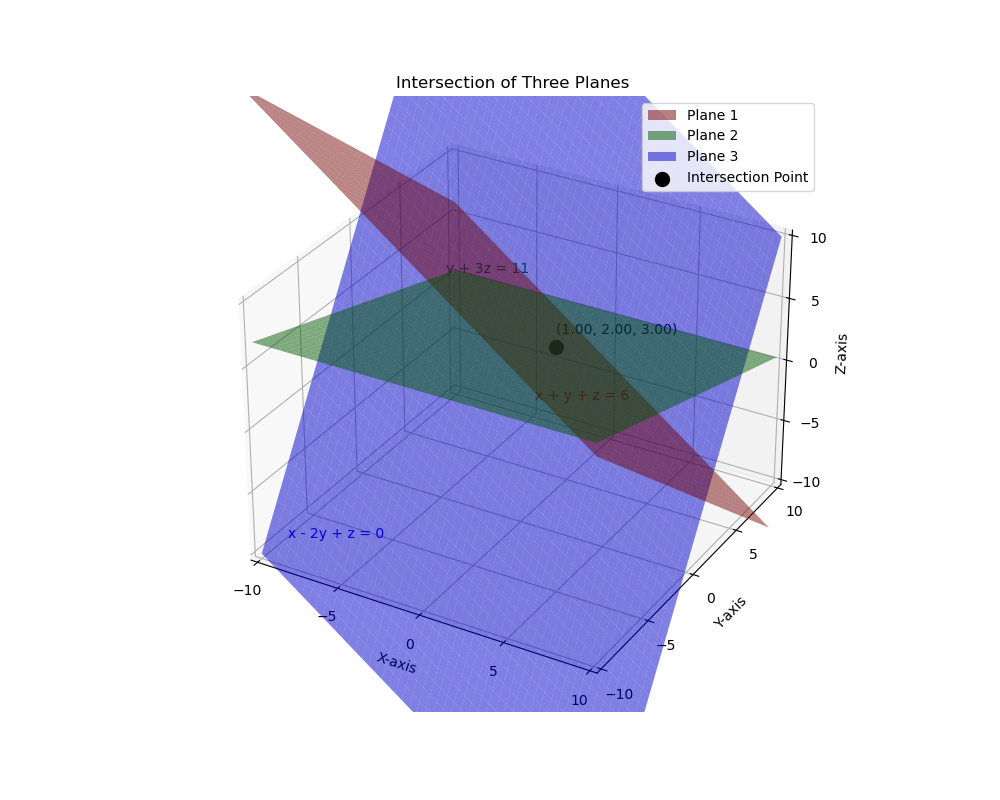
\includegraphics[width=\columnwidth]{figs/fig.png}
\end{center}
\caption{A plane passing through point A with normal vector n.}
\label{fig:Fig.1}
\end{figure}




\end{document}

